\documentclass{beamer}
\usepackage[brazilian]{babel}
\usepackage[utf8]{inputenc}
\usepackage[T1]{fontenc}
\usetheme{Laughlin}
\begin{document}
\title{Algoritmo não Supervisionado para Segmentação e Remoção de
Ruído de Páginas \textit{web} Utilizando \textit{tag paths}}
%\author[Roberto Panerai Velloso]{Orientando: Roberto Panerai Velloso \\
%Orientadora: Carina F. Dorneles \\ \{rvelloso, dorneles\}@gmail.com }
\author[Roberto Panerai Velloso]{Roberto Panerai Velloso, Carina F. Dorneles \\ 
\{rvelloso, dorneles\}@gmail.com}
%\date{\today}
\date{}
%\institute{Universidade Federal de Santa Catarina}
\institute{
%UFSC - Universidade Federal de Santa Catarina \\ PPGCC - Programa de
% Pós-Graduação em Ciência da Computação
\begin{figure}[H]
  \label{fig:logo1}
    
\includegraphics[scale=0.50]{brasao_ufsc_80.png}
    
\includegraphics[scale=0.30]{brasao_418.jpg}
\end{figure}
%\begin{figure}[H]
%  \label{fig:logo2}
%    
\includegraphics[scale=0.30]{brasao_ufsc_80.png}
%\end{figure}
}

\frame{
\titlepage
} 

\frame{\frametitle{Sumário}\tableofcontents}

\section{Introdução} 
%\frame{\tableofcontents[currentsection]}
\frame{\frametitle{Introdução}
\begin{itemize} 
	\item Data mining na web (relevância);
	\begin{itemize}
	\item Usage mining (sistemas de recomendação);
	\item IR (indexing, clustering \& Análise de hyperlinks);
	\item Extração estruturada.
	\end{itemize}
	\item Contexto do trabalho;
	\item Extração estruturada;
	\item Remoção de ruído (importância).
\end{itemize}
}

\frame{\frametitle{Problema}
\begin{itemize} 
	\item Ruído: anúncios, menus, $template$, etc;
	\item Identificar a região principal de uma página $web$, com o objetivo de
	eliminar o restante da página (ruído) antes da fase de extração dos dados;
	\item Etapa de limpeza é fundamental para obtenção de resultados satisfatórios
	na fase de extração de dados;
	\item Poucos trabalhos na área (LIU; CHANG, 2004).
\end{itemize}
}

\frame{\frametitle{Problema}
\begin{figure}[H]
  \caption{Exemplo de uma página web com a região principal delimitada
  HTML.}
  \label{fig:ex2}
  \centering
    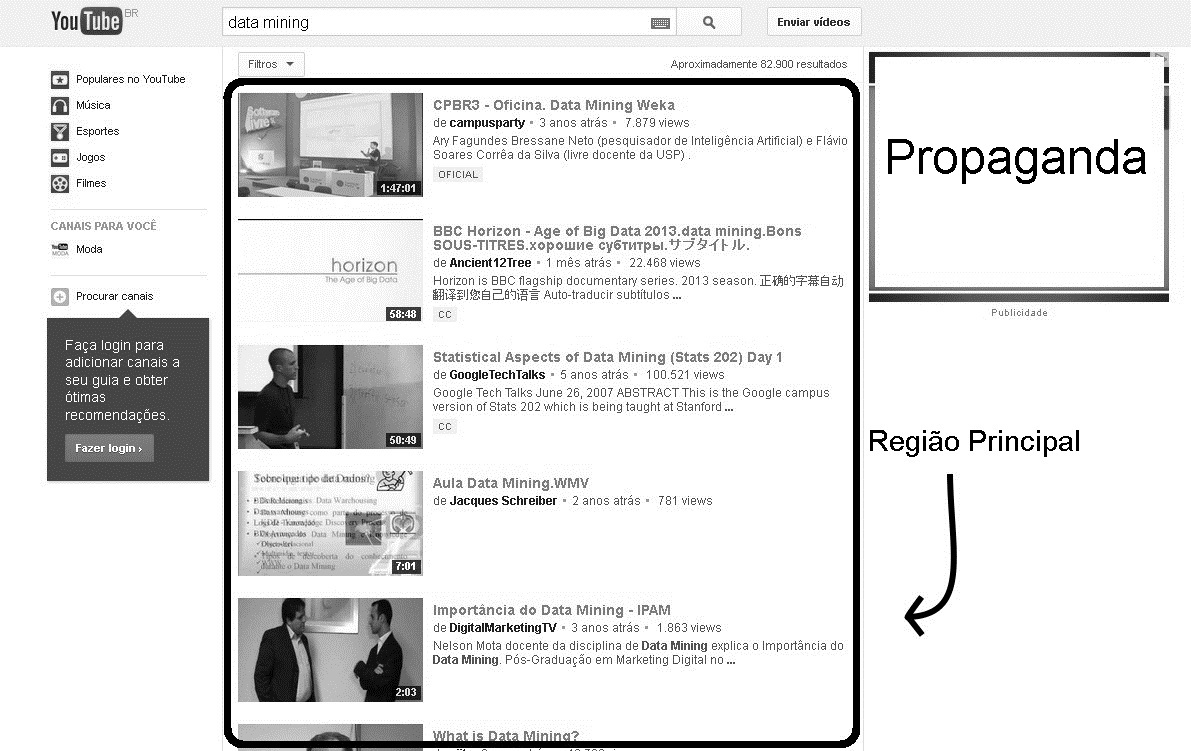
\includegraphics[scale=0.29]{example2-gs-pt.jpg}
\end{figure}
}

\section{Objetivo} 
%\frame{\tableofcontents[currentsection]}
\frame{\frametitle{Objetivo} 
Contribuir para a área de extração estruturada de dados da $web$ com uma nova
técnica de remoção de ruído que possibilite incrementar a precisão dos métodos
de extração e que tenha as seguintes características:
\begin{itemize}
  \item Independente de domínio;
  \item Independente de características da linguagem HTML; 
  \item Totalmente automática;
  \item Necessite de apenas uma página (ao invés de um conjunto de páginas);
  \item Não dependa de treinamento;
  \item Não dependa de bases de dados e/ou definições $a$ $priori$.
\end{itemize}
}
\section{Trabalhos correlatos} 
%\frame{\tableofcontents[currentsection]}
\frame{\frametitle{Trabalhos correlatos} 
\begin{itemize}
	\item Técnicas baseadas no conteúdo textual
		\begin{itemize}
			\item (KOHLSCHÜTTER; NEJDL, 2008; KOHLSCHÜTTER; FANKHAUSER; NEJDL, 2010;
			WENINGER; HSU; HAN, 2010; FERNANDES et al., 2007)
		\end{itemize}
	\item Técnicas baseadas no DOM
		\begin{itemize}
			\item (CHO; LIN; KAO, 2009; FERNANDES et al., 2011; CHAKRABARTI; KUMAR;
			PUNERA, 2008; YI; LIU; LI, 2003; ZHENG; GU; LI, 2012)
		\end{itemize}
	\item Técnicas baseadas em informação visual
		\begin{itemize}
			\item (CAI et al., 2003; LIU; MENG; MENG, 2009; SIMON; LAUSEN, 2005)
		\end{itemize}
	\item $Tag$ $paths$
		\begin{itemize}
			\item (MIAO et al., 2009; XIE; FANG; ZHANG, 2012)
		\end{itemize}
\end{itemize}
}
\subsection{$Tag$ $paths$}

\frame{\frametitle{$Tag$ $paths$}
\begin{figure}[H]
  \caption{Exemplo de uma seqüência de $tag$ $paths$ (TPS) construída a partir de código
  HTML.}
  \label{fig:ex1}
  \centering
    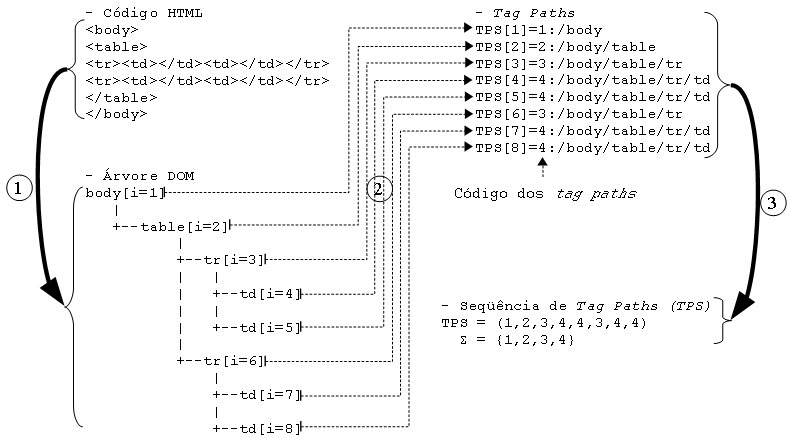
\includegraphics[scale=0.45]{example1-pt.jpg}
\end{figure}
}
\section{Hipótese} 
%\frame{\tableofcontents[currentsection]}
\frame{\frametitle{Hipótese}
\begin{enumerate}
	\item Diferentes regiões de uma página $web$ são descritas utilizando diferentes
	$tag$ $paths$;
	\item Em páginas com conteúdo semi-estruturado (i.e. registros, como definido
	em (LIU; GROSSMAN; ZHAI, 2003)), a região principal é estruturalmente mais
	densa/maior que as demais regiões da página (menus, anúncios, texto, etc.).
\end{enumerate} 
}
\subsection{Algoritmo}

\frame{\frametitle{Algoritmo}
\begin{figure}[H]
  \caption{Ilustração da execução do algoritmo.}
  \label{fig:alg}
  \centering
    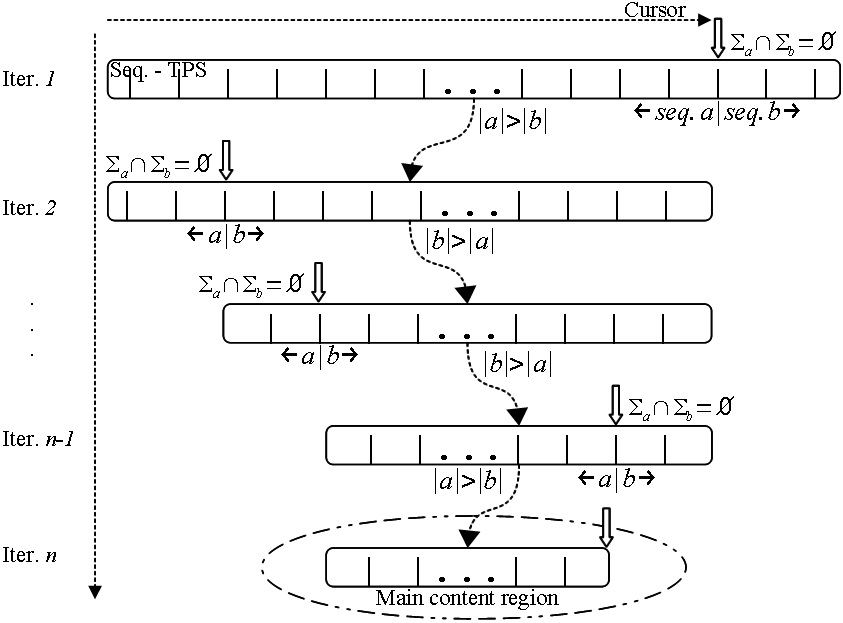
\includegraphics[scale=0.36]{alg-pb.jpg}
\end{figure}
}

\frame{\frametitle{Algoritmo}
\begin{figure}[H]
  \caption{Detecção da região principal em uma página web real.}
  \label{fig:alg}
  \centering
    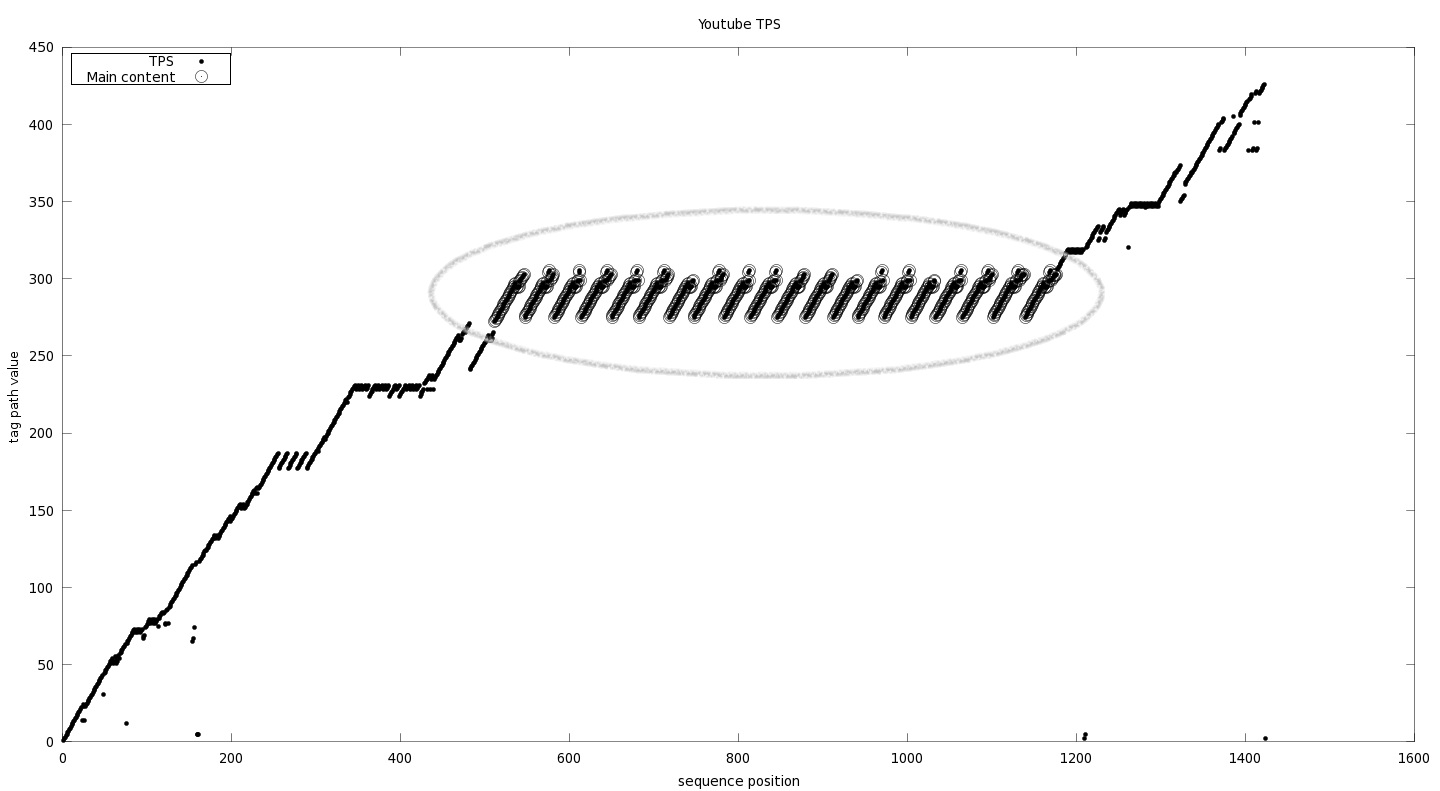
\includegraphics[scale=0.24]{tps.jpg}
\end{figure}
}

\begin{frame}[fragile]
\frametitle{Algoritmo}
\fontsize{8}{7.2}\selectfont
\begin{itemize}
\item{HTML code} 
\begin{verbatim}
<body>
<br>
<div>
  <span class='region1'></span>
  ...
  <span class='region1'></span>
</div> 
<div>
  <span class='region2'></span>
  ...
  <span class='region2'></span>
</div>
<div>
  <span class='region3'></span>
  ...
  <span class='region3'></span>
</div>
<br>
</body>
\end{verbatim}
\item{TPS}
\begin{verbatim}
TPS = (1,2,3,4,...,4,3,5,...,5,3,6,...,6,2)
\end{verbatim}
\item{TPS filtrada}
\begin{verbatim}
TPS = ( , , ,4,...,4, ,5,...,5, ,6,...,6, )
\end{verbatim}
\end{itemize}
\end{frame}

\section{Método} 
%\frame{\tableofcontents[currentsection]}
\frame{\frametitle{Método}
\begin{enumerate}
	\item Escolha de uma técnica de extração estruturada: MDR (LIU; GROSSMAN;
	ZHAI, 2003);
	\item Definição de um conjunto de páginas para teste;
	\item Aplicação da técnica de extração no conjunto de teste, documentando os
	resultados obtidos como $target$ (registro de interesse) ou $noise$
	(ruído);
	\item Nova aplicação da técnica de extração no mesmo conjunto de teste, mas
	desta vez filtrando-o antes, utilizando a técnica proposta neste trabalho,
	documentando os resultados da mesma maneira;
	\item Comparação de ambos os resultados e medição do aumento/redução da
	precisão (remoção de ruído).
\end{enumerate} 
}

\frame{\frametitle{Método}
\begin{figure}[H]
  \caption{Método de avaliação e comparação dos resultados.}
  \label{fig:alg}
  \centering
    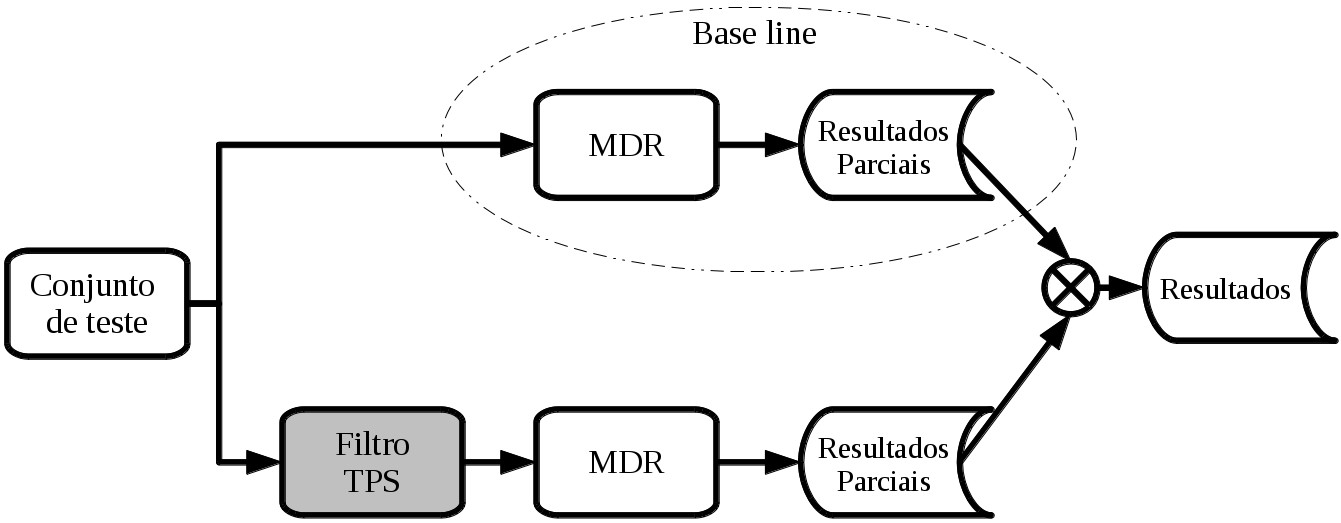
\includegraphics[scale=0.20]{metodo.jpg}
\end{figure}
}

\section{Resultados} 
%\frame{\tableofcontents[currentsection]}
\frame{\frametitle{Resultados} 
\begin{figure}[H]
  \label{fig:res}
  \centering
    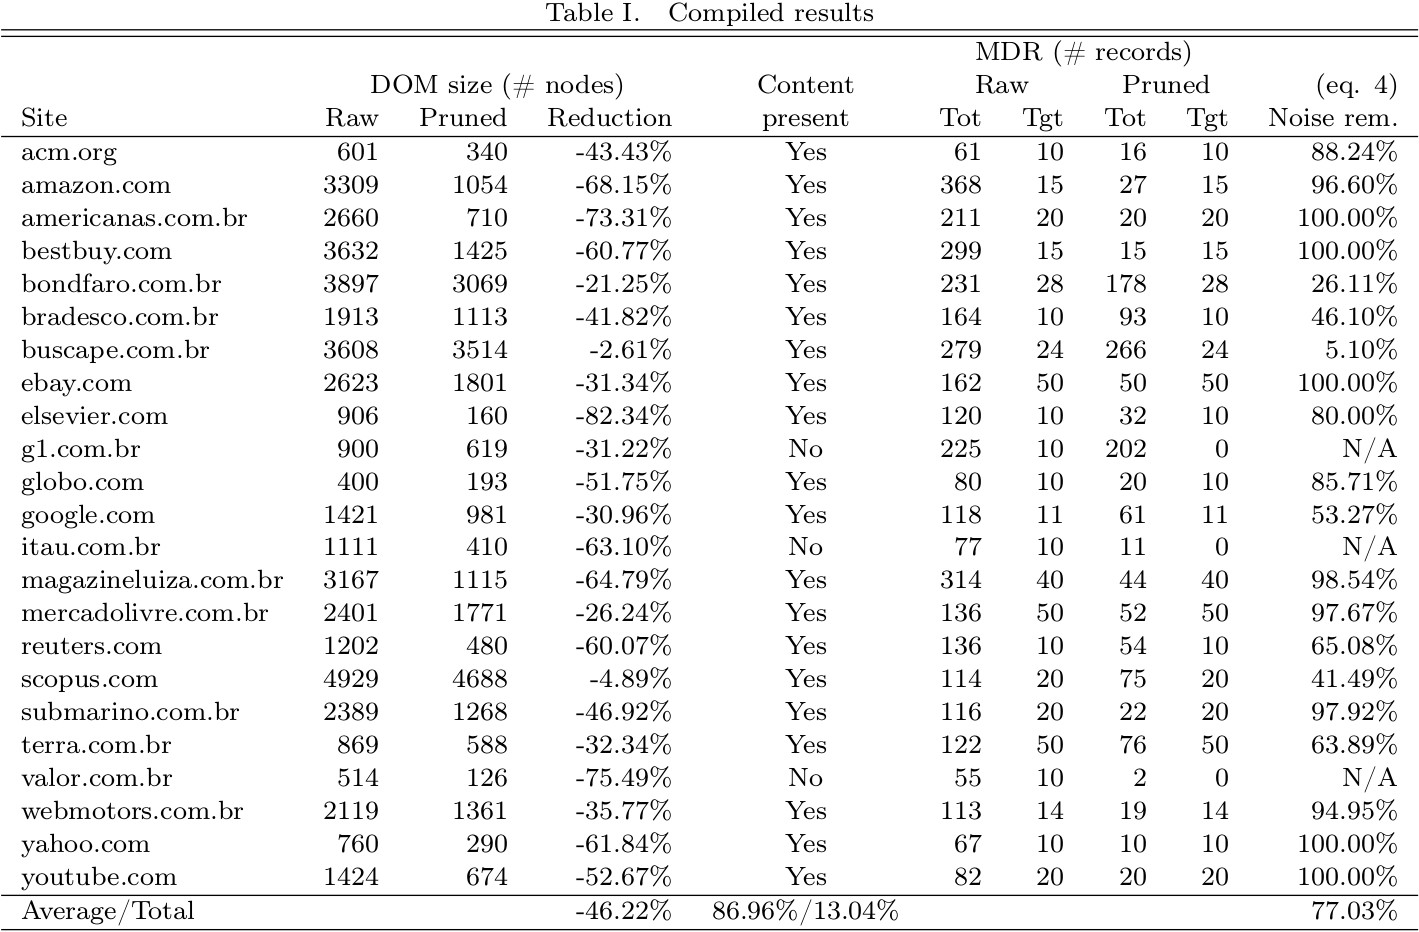
\includegraphics[scale=0.18]{result.jpg}
\end{figure}
}

\section{Limitações} 
%\frame{\tableofcontents[currentsection]}
\frame{\frametitle{Limitações}
\begin{itemize}
	\item Páginas muito homogêneas;
	\item Páginas muito heterogêneas;
	\item Páginas onde o conteúdo principal é menor que o ruído.
\end{itemize}
}

\section{Trabalhos futuros}
%\frame{\tableofcontents[currentsection]}
\frame{\frametitle{Trabalhos futuros}
\begin{itemize}
  \item Combinar com outras abordagens (semânticas);
  \item Generalizar mais a hipótese sobre páginas com conteúdo estruturado. 
\end{itemize}
}

\section{Referências} 
%\frame{\tableofcontents[currentsection]}
\frame{\frametitle{Referências}
\fontsize{8}{7.2}\selectfont
\begin{itemize} 
	\item CAI, D. et al. Extracting content structure for web pages based on visual
	representation. In: Web Technologies and Applications. [S.l.]: Springer, 2003.
	(5th Asia-Pacific Web Conference, APWeb 2003, Xian, China, April 23-25, 2003
	Proceedings), cap. Session 9, p. 406-417.
	\item CHAKRABARTI, D.; KUMAR, R.; PUNERA, K. A Graph-Theoretic Approach to
	Webpage Segmentation. Proceedings of the International World Wide Web
	Conferences, 2008.
	\item CHO, W.-T.; LIN, Y.-M.; KAO, H.-Y. Entropy-based Visual Tree Evaluation 
	on Block Extraction. IEEE/WIC/ACM International Conference on Web Intelligence
	and Intelligent Agent Technology, 2009.
	\item FERNANDES, D. et al. Computing Block Importance for Searching on Web
	Sites. Proceedings of the International Conference on Information and Knowledge
	Engineering, 2007.
	\item FERNANDES, D. et al. A Site Oriented Method for Segmenting Web Pages.
	Proceedings of the International ACM SIGIR Conference on Research \&
	Development of Information Retrieval, 2011.
	\item KOHLSCHÜTTER, C.; FANKHAUSER, P.; NEJDL, W. Boilerplate Detection using
	Shallow Text Features. International Conferences on Web Search and Data Mining,
	2010.
	\item KOHLSCHÜTTER, C.; NEJDL, W. A Densitometric Approach to Web Page
	Segmentation. Proceedings of the International Conference on Information and
	Knowledge Engineering, 2008.
	\item LIU, B.; CHANG, K. C.-C. Editorial: Special Issue on Web Content Mining.
	Proceedings of the ACM SIGKDD International Conference on Knowledge Discovery
	and Data Mining, 2004.
\end{itemize}
}

\frame{\frametitle{Referências}
\fontsize{8}{7.2}\selectfont
\begin{itemize} 
	\item LIU, B.; GROSSMAN, R.; ZHAI, Y. Mining Data Records in Web Pages.
	Proceedings of the ACM SIGKDD International Conference on Knowledge Discovery
	and Data Mining, 2003.
	\item LIU, W.; MENG, X.; MENG, W. ViDE: A Vision-Based Approach for Deep Web
	Data Extraction. IEEE Transactions on Knowledge and Data Engineering, 2009.
	\item MIAO, G. et al. Extracting Data Records from the Web Using Tag Path
	Clustering. Proceedings of the International World Wide Web Conferences, 2009.
	\item SIMON, K.; LAUSEN, G. ViPER: Augmenting Automatic Information Extraction
	with Visual Perceptions. Proceedings of the International Conference on
	Information and Knowledge Engineering, 2005.
	\item WENINGER, T.; HSU, W. H.; HAN, J. CETR - Content Extraction via Tag
	Ratios. Proceedings of the International World Wide Web Conferences, 2010.
	\item XIE, X.; FANG, Y.; ZHANG, L. L. Z. Extracting Data Records from Web Using
	Sux Tree. Proceedings of the ACM SIGKDD International Conference on Knowledge
	Discovery and Data Mining, 2012.
	\item YI, L.; LIU, B.; LI, X. Eliminating Noisy Information in Web Pages for
	Data Mining. Proceedings of the ACM SIGKDD International Conference on
	Knowledge Discovery and Data Mining, 2003.
	\item ZHENG, X.; GU, Y.; LI, Y. Data Extraction from Web Pages Based on
	Structural-Semantic Entropy. Proceedings of the International World Wide Web
	Conferences, 2012.
\end{itemize}
}
\end{document}
